\newif\ifglobal

%%%%%%%%%%%%%%%%%%%%%%%
%%% Compile to view %%%
%%%%%%%%%%%%%%%%%%%%%%%

%%%%%%%%%%%%%%%%%%%%%%%%%%%%%%%%%%%%%%%%%%%%%%%%%%%
%%% Readme:                                     %%%
%%% https://www.overleaf.com/read/bwdjvfjksvjy/ %%%
%%%%%%%%%%%%%%%%%%%%%%%%%%%%%%%%%%%%%%%%%%%%%%%%%%%

% >>> M?: marks a module setting number or important notice

% >>> M4: Set {./relative-path} to external files for this module <<<
\def \modulefiles {./10-BOOTCTRL}
% To add an external file, use:
% (Replace '---' with actual filename)
% '\input{\modulefiles/tables/---.tex}' for tables
% '\includegraphics{\modulefiles/figures/---}' for figures
% '\subfile{\modulefiles/---}' for register files


% >>> M1: This module is in global project? <<<
% 'YES' - uncomment; 'NO' - comment out
\globaltrue

\ifglobal
    \documentclass[main\_\_EN.tex]{subfiles}

\else
    \documentclass[openany, 10pt]{book}

    % >>> M2: In ./00-shared/preamble-trm-module, also find
    %         settings for visibility of todo notes, watermark <<<
    \usepackage{preamble-trm-module}

    % >>> M3: Temporary labels in English,
    %         you can add your own labels there <<<
    \myexternaldocument{./00-shared/temp-labels-en}

\fi %\ifglobal


\setcounter{secnumdepth}{4}


% >>> M5: If this module needs any updates in
% './00-shared/preamble-trm-module.sty'
% (include additional package, etc.), contact your module PM
% or create the file './00-shared/changelog.tex' make the
% necessary updates yourself and document them in this file <<<


\begin{document}


% Sets language into which pre-defined bits of text are translated
\selectlanguage{english}

% Do not delete this block
\ifglobal
% Add the following front matter if
% this module is outside of global project
\else
    \InputIfFileExists{readme}{}{}
    {\let\clearpage\relax \listoftodos}
    {\let\clearpage\relax \listofdonetodos}
    \tableofcontents
    %\listoftables
    %\listoffigures
\fi


%%%%%%%%%%%%%%%%%%%%%%%%%
%%% TRM Module Begins %%%
%%%%%%%%%%%%%%%%%%%%%%%%%

\hypertarget{bootctrl}{}
\chapter{Chip Boot Control}
\label{mod:bootctrl}


\section{Overview}

Chip boot process and some chip functions are determined on power-on or hardware reset using strapping pins and eFuses. The following functionality can be determined:
\begin{itemize}
    \item chip boot mode
    \item enable or disable of ROM messages printing to UART0
    \item source of JTAG signals
    \item SDIO input sampling edge and output driving edge

\end{itemize}

\chipname{} has five strapping pins:
\begin{itemize}
    \item MTMS
    \item MTDI
    \item GPIO8
    \item GPIO9
    \item GPIO15
\end{itemize}


During Chip Reset (see Chapter \ref{mod:resclk} \textit{\nameref{mod:resclk}}), hardware captures samples and stores the voltage level of strapping pins as strapping bit of ``0" or ``1" in latches, and holds these bits until the chip is powered down or the next chip reset. Software can read the latch status (strapping value) from \hyperref[fielddesc:GPIOSTRAPPING]{GPIO\_STRAPPING}.

\section{Functional Description}

This section provides description of the chip functions and the patterns of the strapping pins and eFuse values to invoke each function.

\begin{importantlisting}

Only documented patterns should be used. If an undocumented pattern is used, it may trigger unexpected behaviors.
\end{importantlisting}

\subsection{Default Configuration}
By default, GPIO9 is connected to the chip's internal pull-up resistor. If GPIO9 is not connected or is connected to an external high-impedance circuit, the internal weak pull-up determines the default input level of this strapping pin (see Table \ref{tab:bootctrl-default-config-strapping-pins}).

\clearpage
\begin{longtable}[c]{|p{2.5cm}|p{3.5cm}|}
\caption{Default Configuration of Strapping Pins}
\label{tab:bootctrl-default-config-strapping-pins} \\
    \hline
    \rowcolor{lightgray}
  \textbf{Strapping Pin} & \textbf{Default Configuration} \\ \hline
  \textbf{MTMS} & Floating \\ \hline
  \textbf{MTDI} & Floating \\ \hline
  \textbf{GPIO8} & Floating \\ \hline
  \textbf{GPIO9} & Pull-up \\ \hline
  \textbf{GPIO15} & Floating \\ \hline
\end{longtable}
To change the strapping bit values, users can apply external pull-down/pull-up resistors, or use host MCU GPIOs to control the voltage level of these pins when powering on \chipname{}. After the reset is released, the strapping pins work as normal-function pins.

\subsection{Boot Mode Control}\label{sec:bootModeControl}

The values of GPIO8 and GPIO9 at reset determine the boot mode after the reset is released. Table \ref{tab:bootctrl-boot-mode-control} shows the strapping pin values of GPIO8 and GPIO9, and the associated boot modes.

\begin{ThreePartTable}

\begin{TableNotes}
    \item[*] x: this value is ignored.
\end{TableNotes}
\begin{longtable}[c]{|p{2.5cm}|c|c|c|}
\caption{Boot Mode Control}
\label{tab:bootctrl-boot-mode-control} \\
    \hline
    \rowcolor{lightgray}
  \textbf{Boot Mode} & \textbf{GPIO9} & \textbf{GPIO8}\\
    \hline
    \endfirsthead
    \insertTableNotes
    \endlastfoot
  SPI Boot & 1 & x \\ \hline
  Download Boot & 0 & 1\\ \hline
\end{longtable}
\end{ThreePartTable}

In SPI Boot mode, the ROM bootloader loads and executes the program from SPI flash to boot the system.
SPI Boot mode can be further classified as follows:
\begin{itemize}
    \item Normal Flash Boot: supports Secure Boot. The ROM bootloader loads the program from flash into SRAM and executes it. In most practical scenarios, this program is the 2nd stage bootloader, which later boots the target application.
    \item Direct Boot: does not support Secure Boot and programs run directly from flash. To enable this mode, make sure that the first two words of the bin file downloaded to flash are 0xaedb041d. For more detailed process, see Figure \ref{fig:boot_flow}.
\end{itemize}
In Download Boot mode, users can download code into flash using UART0 or USB interface. It is also possible to load a program into SRAM and execute it from SRAM.

Figure \ref{fig:boot_flow} shows the detailed boot flow of the chip.

\begin{figure}[H]
    \centering
    {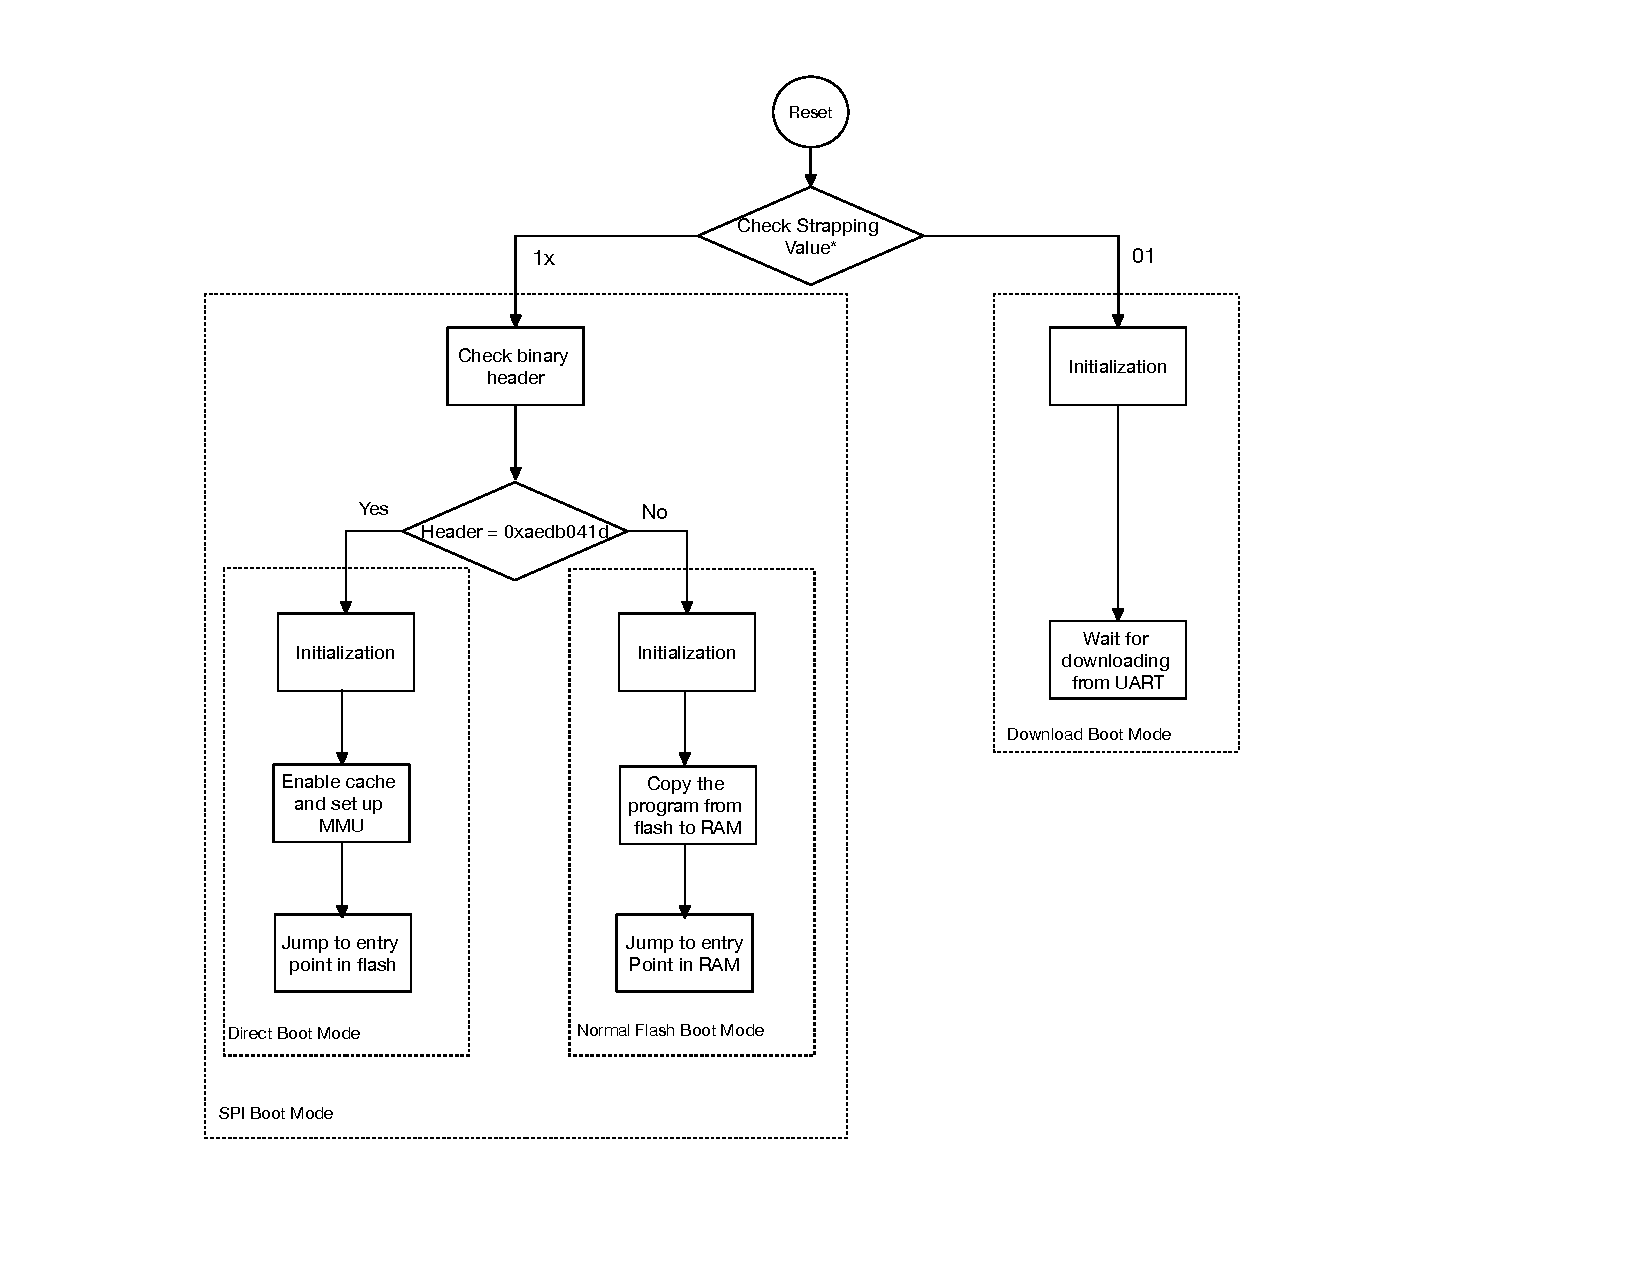
\includegraphics[width=1.0\textwidth]{10-BOOTCTRL/figures/boot_flow_20220728.pdf}}\\
    \textbf{*Note}: The strapping values "1x" and "01" are the combination of GPIO9 and GPIO8 pins, see Table \ref{tab:bootctrl-boot-mode-control}.
    \caption{Chip Boot Flow}
    \label{fig:boot_flow}
\end{figure}

The following eFuses allows controlling boot mode behaviors:

\begin{itemize}
    \item \hyperref[fielddesc:EFUSEDISFORCEDOWNLOAD]{EFUSE\_DIS\_FORCE\_DOWNLOAD}
    \begin{itemize}
    \item If this eFuse is 0 (default), software can force switch the chip from SPI Boot mode to Download Boot mode by setting register \hyperref[fielddesc:LPAONFORCEDOWNLOADBOOT]{LP\_AON\_FORCE\_DOWNLOAD\_BOOT} and triggering a CPU reset.  In this case, hardware overwrites \hyperref[fielddesc:GPIOSTRAPPING]{GPIO\_STRAPPING}[3:2] from ``1x" to ``01".
    \item If this eFuse is 1, \hyperref[fielddesc:LPAONFORCEDOWNLOADBOOT]{LP\_AON\_FORCE\_DOWNLOAD\_BOOT} is disabled. \hyperref[fielddesc:GPIOSTRAPPING]{GPIO\_STRAPPING} can not be overwritten.
    \end{itemize}

    \item \hyperref[fielddesc:EFUSEDISDOWNLOADMODE]{EFUSE\_DIS\_DOWNLOAD\_MODE}

    If this eFuse is 1, Download Boot mode is permanently disabled. \hyperref[fielddesc:GPIOSTRAPPING]{GPIO\_STRAPPING} will not be overwritten by \hyperref[fielddesc:LPAONFORCEDOWNLOADBOOT]{LP\_AON\_FORCE\_DOWNLOAD\_BOOT}.

    \item \hyperref[fielddesc:EFUSEENABLESECURITYDOWNLOAD]{EFUSE\_ENABLE\_SECURITY\_DOWNLOAD}

    If this eFuse is 1, Download Boot mode only allows reading, writing, and erasing plaintext flash and does not support any SRAM or register operations. Ignore this eFuse if Download Boot mode is disabled.

    \item \hyperref[fielddesc:EFUSEDISDIRECTBOOT]{EFUSE\_DIS\_DIRECT\_BOOT}

    If this eFuse is 1, Direct Boot mode is disabled.
\end{itemize}

USB Serial/JTAG Controller can also force switch the chip to Download Boot mode from SPI Boot mode, and vice versa. For detailed information, please refer to Chapter \ref{mod:usbserialjtag} \textit{\nameref{mod:usbserialjtag}}.

\subsection{ROM Messages Printing Control}


During early SPI Boot process the messages by the ROM code can be printed to:

\begin{itemize}
    \item \textbf{(Default) UART0 and USB Serial/JTAG controller}
    \item \textbf{USB Serial/JTAG controller}
    \item \textbf{UART0}
    \end{itemize}

\hyperref[fielddesc:EFUSEUARTPRINTCONTROL]{EFUSE\_UART\_PRINT\_CONTROL} and GPIO8 control ROM messages printing to \textbf{UART0} as shown in Table \ref{tab:bootctrl-rom-code-printing-control} \nameref{tab:bootctrl-rom-code-printing-control}.

\begin{table}[H]
    \centering
    \caption{ROM Message Printing Control}
    \label{tab:bootctrl-rom-code-printing-control}
    \begin{threeparttable}
    \begin{tabular}{ |p{1.3cm}<{\centering}|p{1.3cm}<{\centering}|p{9cm}|}
    \hline
        \rowcolor{lightgray}
    \textbf{eFuse\tnote{1}} &   \textbf{GPIO8}      & \textbf{ROM Code Printing} \\\hline
    0 &  x  & Always enabled \\\hline
    \multirow{2}*{1}   & 0     & Enabled\\\cline{2-3}
     & 1       & Disabled \\\hline
    \multirow{2}*{2}   & 0     & Disabled \\\cline{2-3}
     & 1       & Enabled\\\hline
     3 & x  & Always disabled \\\hline
        \end{tabular}

        \begin{tablenotes}
            \item[1] eFuse: \hyperref[fielddesc:EFUSEUARTPRINTCONTROL]{EFUSE\_UART\_PRINT\_CONTROL}
        \end{tablenotes}
     \end{threeparttable}
    \end{table}

\hyperref[fielddesc:EFUSEDISUSBSERIALJTAGROMPRINT]{EFUSE\_DIS\_USB\_SERIAL\_JTAG\_ROM\_PRINT} controls the printing to \textbf{USB Serial/JTAG controller}. When this bit is 1, printing to USB Serial/JTAG controller is disabled. When this bit is 0, and USB Serial/JTAG controller is enabled via \hyperref[fielddesc:EFUSEDISUSBSERIALJTAG]{EFUSE\_DIS\_USB\_SERIAL\_JTAG}, ROM messages can be printed to USB Serial/JTAG controller.


Note that if \hyperref[fielddesc:EFUSEDISUSBSERIALJTAGROMPRINT]{EFUSE\_DIS\_USB\_SERIAL\_JTAG\_ROM\_PRINT} is set to 0 to print to USB, but USB Serial/JTAG Controller has been disabled, then ROM messages will not be printed to USB Serial/JTAG Controller.

\subsection{JTAG Signal Source Control}

GPIO15 controls the source of JTAG signals during the early boot process. This GPIO is used together with \hyperref[fielddesc:EFUSEDISPADJTAG]{EFUSE\_DIS\_PAD\_JTAG}, \hyperref[fielddesc:EFUSEDISUSBJTAG]{EFUSE\_DIS\_USB\_JTAG}, and \hyperref[fielddesc:EFUSEJTAGSELENABLE]{EFUSE\_JTAG\_SEL\_ENABLE}. See Table \ref{tab:bootctrl-jtag-signal-src-control}.

\begin{table}[H]
    \centering
    \caption{JTAG Signal Source Control}
    \label{tab:bootctrl-jtag-signal-src-control}
    \begin{threeparttable}
    \begin{tabular}{ |p{1.3cm}<{\centering}|p{1.3cm}<{\centering}|p{1.3cm}<{\centering}|p{1.5cm}<{\centering}|p{8.0cm}| }
    \hline
        \rowcolor{lightgray}
        \textbf{eFuse 1\tnote{a}} & \textbf{eFuse 2\tnote{b}} & \textbf{eFuse 3\tnote{c}} &   \textbf{GPIO15}      & \textbf{Signal Source} \\\hline
    \multirow{3}*{0} & \multirow{3}*{0} & 0 &  x  & JTAG signals come from USB Serial/JTAG Controller.\\\cline{3-5}
    & & \multirow{2}*{1}   & 0     & JTAG signals come from corresponding pins\tnote{d}.  \\\cline{4-5}
    & & & 1       & JTAG signals come from USB Serial/JTAG Controller. \\\hline
    0 & 1 & x & x & JTAG signals come from corresponding pins\tnote{d}.\\\hline
    1 & 0 & x & x & JTAG signals come from USB Serial/JTAG Controller. \\\hline
    1 & 1 & x & x & JTAG is disabled.\\\hline
        \end{tabular}

        \begin{tablenotes}
            \item[a] eFuse 1: \hyperref[fielddesc:EFUSEDISPADJTAG]{EFUSE\_DIS\_PAD\_JTAG}
            \item[b] eFuse 2: \hyperref[fielddesc:EFUSEDISUSBJTAG]{EFUSE\_DIS\_USB\_JTAG}
            \item[c] eFuse 3: \hyperref[fielddesc:EFUSEJTAGSELENABLE]{EFUSE\_JTAG\_SEL\_ENABLE}
            \item[d] JTAG pins: MTDI, MTCK, MTMS, and MTDO
        \end{tablenotes}
     \end{threeparttable}
    \end{table}

\subsection{SDIO Sampling Input Edge and Output Driving Edge Control}

The strapping pin MTMS and MTDI can be used to control the input sampling edge and the output driving edge. See Table \ref{tab:2.8-sdio-strapping} \nameref{tab:2.8-sdio-strapping}. For more information about SDIO sampling control, see Chapter \ref{mod:sdioslave} \textit{\nameref{mod:sdioslave}}.



        % table contents

\begin{table}[H]
    \centering
    \caption{SDIO Input Sampling Edge/Output Driving Edge Control}
   \label{tab:2.8-sdio-strapping}

    \begin{threeparttable}
    \begin{tabular}{ | p{1.8cm}<{\centering} | p{1.8cm}<{\centering} | p{6.8cm}| }
    \hline
        \rowcolor{lightgray}
        \textbf{MTMS} & \textbf{MTDI} & \textbf{Edge behavior} \\\hline

        % table contents
        0 & 0 & Falling edge sampling, falling edge output \\\hline
        0 & 1 & Falling edge sampling, rising edge output \\\hline
        1 & 0 & Rising edge sampling, falling edge output \\\hline
        1 & 1 & Rising edge sampling, rising edge output \\\hline
        \end{tabular}
     \end{threeparttable}
\end{table}
\end{document}
